%=================================================================
\chapter{IMPLEMENTACI\'ON DE LA PROPUESTA} \label{cha:implementacion}
%=================================================================

Kalcas fue desarrollado con el IDE Eclipse y construido sobre Eclipse Modelling Framework (EMF). Toda la implementaci\'on se divide en seis grupos de proyectos Eclipse que se muestran en la Figura \ref{fig:projects}. El primer proyecto contiene el metamodelo ecore de EA. El segundo proyecto \textit{tartarus.serializer} contiene los importadores tanto de procesos de negocio como de esquemas de base de datos. El tercero \textit{tartarus.transformation} contiene las plantillas Xpand que genera los archivos OWL a partir del modelo Tartarus. Los proyectos \textit{co.edu.uniandes.kalcasql} corresponden a los proyectos GMF que generan el editor gr\'afico KQL. El proyecto \textit{co.edu.uniandes.kalcas.tartarus2kalcas} genera el modelo de respuesta para una consulta hecha en KQL. Por \'ultimo, \textit{co.edu.uniandes.kalcas.kalcas2gv} contiene la transformaci\'on XPand que genera el archivo dot a partir de la respuesta generada. La Figura \ref{fig:arch} ofrece una vista general de la arquitectura de Kalcas. A continuaci\'on se explican con mayor detalle los proyectos en que se ha implementado nuestra aproximaci\'on.

%--------------------------------------------------------------------------------------
\begin{figure}[!t]
\begin{center}
	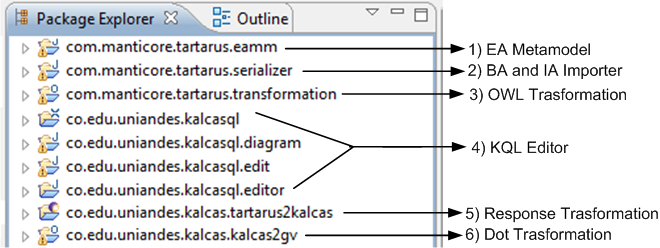
\includegraphics[scale=0.5 ,natwidth=660pt, natheight=248pt]{projects.png}
	\caption{Proyectos Eclipse}
	\label{fig:projects}
\end{center}
\end{figure} 
%--------------------------------------------------------------------------------------

%--------------------------------------------------------------------------------------
\begin{figure}[!t]
\begin{center}
	\includegraphics[scale=0.5 ,natwidth=684pt, natheight=281pt]{kalcas_arch.png}
	\caption{Arquitectura Kalcas}
	\label{fig:arch}
\end{center}
\end{figure} 
%--------------------------------------------------------------------------------------


\begin{enumerate}

\item El proyecto \textit{tartarus.eamm} contiene el metamodelo ecore de Tartarus y los modelos xmi conformes a Tartarus. Adicionalmente, en este proyecto tambi\'en est\'an las clases java que representan los conceptos del metamodelo y permiten leer y editar program\'aticamente los modelos conformes con Tartarus. Este proyecto tambi\'en incluye el paquete \textit{matching.align} el cual funciona como interfaz con el motor de alineamiento \textit{AlignmentAPI}. Sobre el archivo \textit{matching.properties} se configuran la ruta de las ontolog\'ias a procesar y el modelo Tartarus donde se registrar\'an los mapeos inferidos. Dentro de este proyecto tambi\'en se encuentra el paquete java \textit{kalcas.verification} que implementa una GUI utilizando la librer\'ia \textit{javax.swing}. Esta GUI permite a un usuario confirmar los mapeos inferidos.

\item Los importadores de BA e IA se localizan en el proyecto \textit{tartarus.serializer}. Clases Java utilizan el API Xstream para acceder los archivos XPDL que describen la BA y las procesan para convertirlas en conceptos Tartarus. Para tal fin, un archivo de propiedades (TartarusSerializer.properties) permite definir la ruta de los archivos fuentes y el modelo Tartarus de destino. En el caso de la IA, se accede program\'aticamente a los esquemas a trav\'es de un conector JDBC y la librer\'ia \textit{java.sql}. Los par\'ametros para conectarse a la base de datos son al igual configurados en archivos de propiedades. Estos importadores generan o actualizan el modelo XMI conforme con Tararus con la informaci\'on contenida en procesos y esquemas.

\item Dentro de \texttt{tartarus.transformation} est\'a la plantilla \textit{Process2RDFXML.xpt} en lenguaje Xpand que se encarga de recorrer el modelo Tartarus para generar ontolog\'ias OWL para cada proceso de la BA. Similarmente la plantilla \textit{Schema2RDFXML.xpt} transforma los esquemas y sus entidades en ontolog\'ias OWL.  Cada plantilla es ejecutada mediante un Motor de Workflow de Modelamiento(Modeling Workflow Engine (GenerateOWLFromProcess.mwe y GenerateOWLFromSchema.mwe). Las ontolog\'ias de salida son generadas en la carpeta src-gen/ para ser procesadas posteriormente.

\item Los proyectos \textit{kalcasql} son los que en conjunto implementan el editor KQL. El proyecto \textit{kalcasql} contiene el metamodelo \textit{kalcasql.ecore} y los modelos intermedios GMF. Los proyectos \textit{diagram, edit} y \textit{editor} comprenden las clases java que implementan el plugin KQLEditor y fueron generadas mediante EuGENia. El editor KQL se ejecuta como una instancia eclipse que el usuario utiliza para dise\~nar las consultas.

\item \textit{Tartarus2kalcas} es un proyecto \textit{ATL} que contiene la transformaci\'on \texttt{query2response.atl} la cual toma un modelo Tartarus y un modelo KQLQuery para procesarlos y generar un modelo de salida conforme con el metamodelo KQLResponse. Este modelo de respuesta es transformado a texto posteriormente.

\item El proyecto \textit{kalcas2gv} contiene el metamodelo KQLResponse.ecore y sus diferentes modelos que representan las respuestas generadas a consultas KQL. Adicionalmente, la plantilla \textit{kalcasql2dot.xpt} implementada en XPand se encarga de realizar la transformaci\'on del modelo de respuesta a un archivo dot. Los archivos dot son generados en la carpeta \textit{src-gen}. Cada archivo dot es interpretado por la herramienta Graphviz y presentado en formato gr\'afico.

\end{enumerate}